\documentclass[a4paper,11pt]{article} \usepackage[T1]{fontenc} \usepackage[utf8]{inputenc} \usepackage[francais]{babel}
\usepackage[top=2cm,left=2.5cm,right=2.5cm,bottom=2cm]{geometry} % Géométrie de la page, modifier selon le besoin
\usepackage{lmodern, wrapfig, textcomp, tikz, graphicx, amsmath, tikz-qtree, xcolor,rotating,epic,eepic}
\usepackage[colorlinks,linkcolor=black, urlcolor=blue]{hyperref}
\usepackage[babel=true,kerning=true]{microtype}
\usetikzlibrary{matrix, arrows, calc, shapes.geometric, shapes.misc, shapes.symbols, shapes.arrows, automata,
    through, positioning, scopes, decorations.shapes, decorations.text, decorations.pathmorphing, shadows}
\date{}
\begin{document}
\pagenumbering{gobble}  % Pas de numérotation
    \begin{titlepage}

\includegraphics[scale=0.45]{Public/logo_phelma.pdf}\hfill
\includegraphics[scale=0.55]{Public/logo_robotronik.png}
\begin{center}
    \vspace*{2cm}
    \rule{\linewidth}{0.5mm}\\[0.4cm]
    {\huge\bfseries Demande de reconnaissance pour investissement dans des activités associatives\\
    [0.4cm]}\rule{\linewidth}{0.5mm}\\[1.0cm]
    \large{\textsc{Félix Piédallu}}
    \begin{flushright} \large
        2\ieme Année \\
        Filière \textsc{Pns} \\
        Président du \textsc{Club Robotronik}\\
    \end{flushright}
    \vfill

    \large{\today}
\end{center}
\end{titlepage}
     % Fichier de page de titre
    \tableofcontents        % Table des matières avec liens, générée automatiquement.
\newpage
\pagenumbering{arabic}  % Numérotation de retour !
\part{Informations sur l'Association}
    L'Association Robotronik (appelée aussi le Club Robotronik) a été créée en 2008, suite à la fusion de PG Robotik
    et du Club Électronique.\\

    Le Club a pour vocation tout d'abord de faire découvrir aux étudiants de Phelma les vastes domaines de la Robotique.
    Il organise et participe à quelques événements en-dehors du Club, comme la Fête de la Science qui s'est justement déroulée ces vendredi et samedi.\\

    Il a donc aussi pour but d'être présent aux différentes manifestations telles que la Fête de la Science,
    pour promouvoir la Robotique au public.\\

    L'objectif du Club chaque année est de participer à la Coupe de France de Robotique, qui rassemble près de
    200 équipes de jeunes à La Ferté-Bernard, dans une ambiance conviviale autour de la Coupe.\\

    Le club regroupe aujourd'hui 7 2\iemes{} Année, ainsi qu'une douzaine de 1\ieres{} Année. Il permet, de façon très exceptionnelle, à des élèves extérieurs à participer au travail du club.

\part{Le rôle que j'exerce dans le Club}
    J'exerce le rôle de Président du Club. Mon rôle est d'organiser la communication tant externe qu'interne, tout en supervisant la progression technique des projets.\\

    La communication interne comprend notamment le recrutement des premières années de Phelma, afin de diriger vers le Club ceux qui se sentiraient intéressés par la robotique.

    Il s'agit aussi de faire connaître le Club auprès de tous les élèves et enseignants de Phelma, qui pourraient alors être intéressés de demander de l'aide pour leurs propres projets ou même fournir de l'aide sur certains points techniques et logistiques du Club.

    Nous encadrons aussi un ou deux projets de groupe chaque année, et c'est à moi de les préparer et de les encadrer, avec un autre membre du Club.

    Nous avons comme projet de préparer pour cette année un concours pour les élèves, basé sur les cartes programmables que nous utilisons à partir de cette année dans nos robots : les STM32.\\

    De plus, j'ai à gérer la communication du Club aux sponsors, qui sont une source de support financier et technique non négligeable pour le club. Il s'agit donc de conserver les anciens sponsors et de trouver de nouveaux sponsors prêts à aider une équipe pour la Coupe de France de Robotique.

    Il m'incombe de préparer notre participation, bien sûr aidé par les membres du Club, aux événements tels que la Fête de la Science ou à l'organisation de la Coupe FIRST.

    \begin{figure}[h] \begin{center} 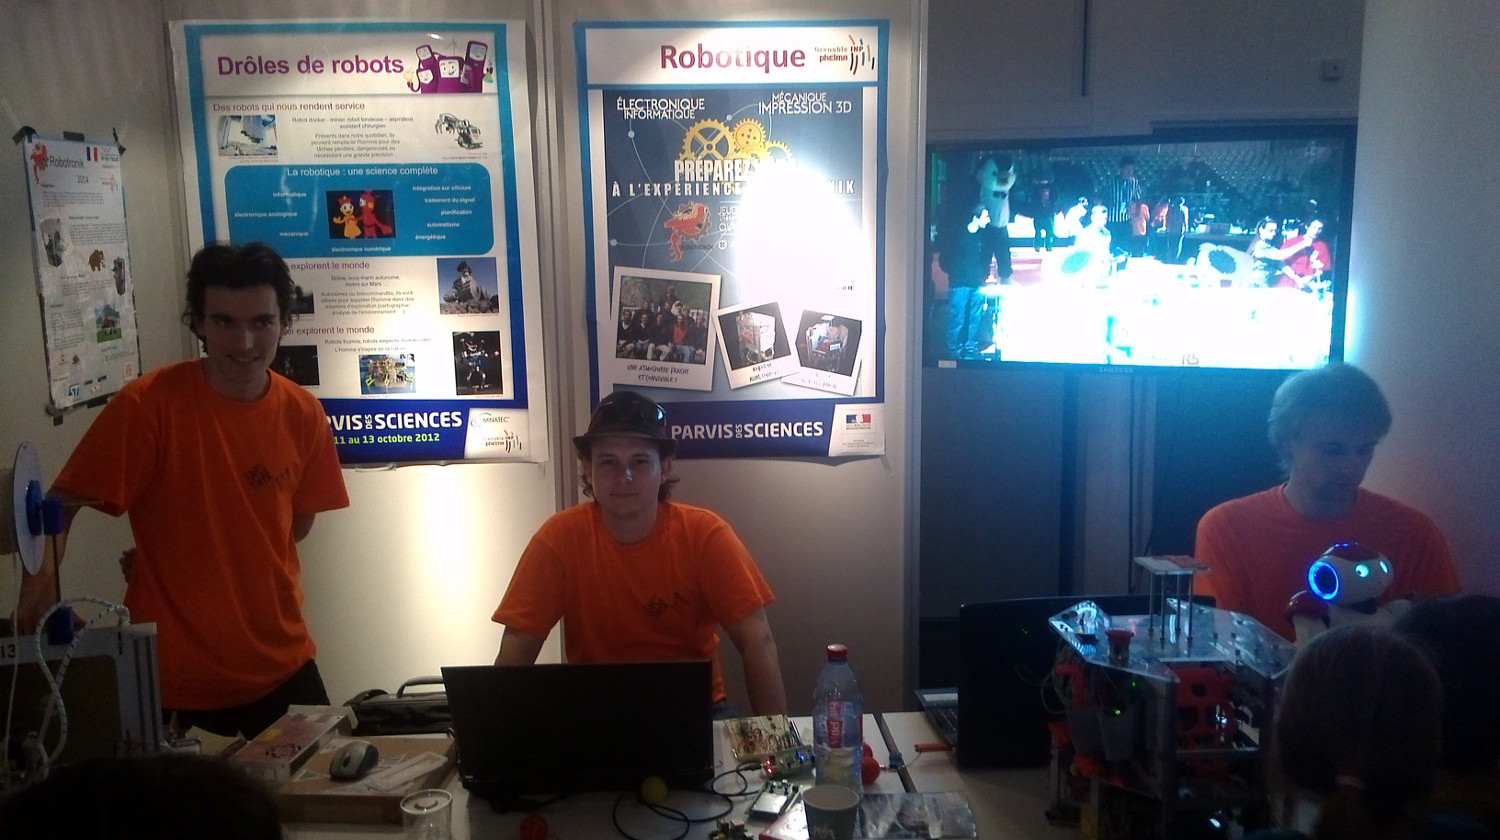
\includegraphics[width=350px]{Images/FeteDeLaScience}
        \caption{Le Stand Robotronik à la Fête de la Science, Samedi 11 Octobre 2014} \end{center} \end{figure}

    Je dois bien sûr m'occuper de l'aspect financier de la gestion du Club, avec le trésorier, Ojeme Ikhalo. Il s'agit donc d'évaluer et de prévoir les besoins du Club.

    De plus, je dois superviser les décisions techniques, afin d'assurer la progression du club. Je suis bien sûr épaulé pour cela du Chef de Projet, Johan Lafon.

\part{Mes objectifs, ceux du Club, et l'objet de ma demande}
Mes objectifs vont bien sûr de pair avec la réussite du Club à la Fête de la Science. Il s'agit donc d'organiser le club afin de mener à terme les différents aspects de la réalisation des robots. Il s'agit aussi de maintenir les partenariats que nous avons afin d'obtenir le soutien nécessaire.\\

En effet cette année, de nombreux changements techniques ont été décidés : des batteries plus performantes mais plus fragiles, de nouvelles cartes programmables -- des STM32 gracieusement fournis par STMicroElectronics -- à maîtriser le plus rapidement possible, ainsi que de nouveaux capteurs d'obstacle -- l'InfraRouge utilisé jusqu'ici nous ayant posé de nombreux problèmes de détection à la Coupe. Tout cela impose de gérer au mieux nos ressources afin de pouvoir maîtriser efficacement ces nouveaux outils, tout en formant les nouveaux membres aux différents aspects de la Robotique et des outils utilisés.\\

De plus, le Club Robotronik participe cette année à de nombreux projets et événements : de l'encadrement de Projets de Groupe à la participation à la Fête de la Science, où nous avons présenté le célèbre Nao d'Aldebaran, et la participation à la création du Char des Ol'INPiades, je dois gérer l'organisation et la présence des membres afin de mener à bien non seulement ces projets, mais aussi la Coupe qui ne doit pas être oubliée parmi les événements.\\

Les aspects événementiels mis à part, je dois m'investir dans la vie du Club, en préparant la séance hebdomadaire du Club du jeudi après-midi, et les soirs où le club est ouvert. Je dois rajouter à cela le temps consacré à l'administration du club, la communication et la prévision des besoins du club.

Cela m'impose de m'investir dans la vie du Club et donc d'être disponible à tout moment pour les membres, ainsi que de connaître parfaitement l'avancement technique du club, auquel je participe bien évidemment.\\

Ma demande s'appuie donc sur le temps que je consacre depuis déjà deux mois au club et les responsabilités qui me sont confiées, mais aussi sur les connaissances que m'apporte cette expérience, qui peut alors se substituer aux cours de Stratégie et Marketing qui m'apportent les mêmes connaissances sans l'expérience.

\part{L'apport d'expérience pour mon futur métier}
    En tant que Président du Club Robotronik, je dois dois encadrer l'équipe du Club, tout en balayant tous les aspects de gestion et d'administration d'une structure équivalente à une Start-Up, avec une échéance à court terme à prévoir, qu'est la Coupe de France.\\

    Tout d'abord la participation au Club Robotronik me permet de découvrir, depuis l'an dernier, le fonctionnement d'une équipe complète, avec un projet de grande envergure, dans ses moindres détails. La gestion du travail d'équipe au sein du club est très formateur, et me permet d'acquérir des compétences essentielles à un ingénieur qui ne peuvent être acquises que par ce type d'expérience.

    Le cahier des charges imposé par l'organisation de la Coupe -- Actions à faire pour gagner des points, limites de dimensions, gestion des robots adverses aussi présents sur le terrain… -- me permet d'apprendre à gérer des contraintes que j'aurai, dans un travail d'ingénieur.\\

    Nous avons pour but d'accueillir de plus en plus de membres au sein du Club, donc en tant que deuxième année, j'ai à gérer plus de nouveaux membres que nous ne sommes d'anciens. Il y a donc un travail d'enseignement énorme. \\
    De plus nous avons à nous former nous-mêmes au nouveaux outils que nous utilisons au club depuis peu. C'est pour cela que j'ai mis en place à la rentrée un Wiki, afin de centraliser les connaissances du club. Ce Wiki est destiné à être rempli par les membres du club, et est laissé ouvert afin de permettre au public de découvrir facilement nos outils.

    De plus j'ai à gérer tous les aspects administratifs et logistiques du club ; ceci fait partie intégrante du travail d'ingénieur ou de chercheur. En effet, mon but est de travailler dans un laboratoire de recherche, j'espère en tant que directeur de recherche, où cet aspect est bien présent ; j'aurai alors déjà acquis les connaissances nécessaires grâce à mon investissement au club Robotronik.

\part{Organisation du Club sur l'année}
Bien sûr, l'échéance principale du Club est la Coupe de France de Robotique, mi-Mai.

Mais nous avons décidé comme échéance idéale la pré-coupe de Lyon qui a lieu en Mars. Cela nous donnera le temps d'améliorer et de paramétrer nos robots en fonction des résultats que nous aurons obtenus.\\
\begin{figure}[h] \begin{center} 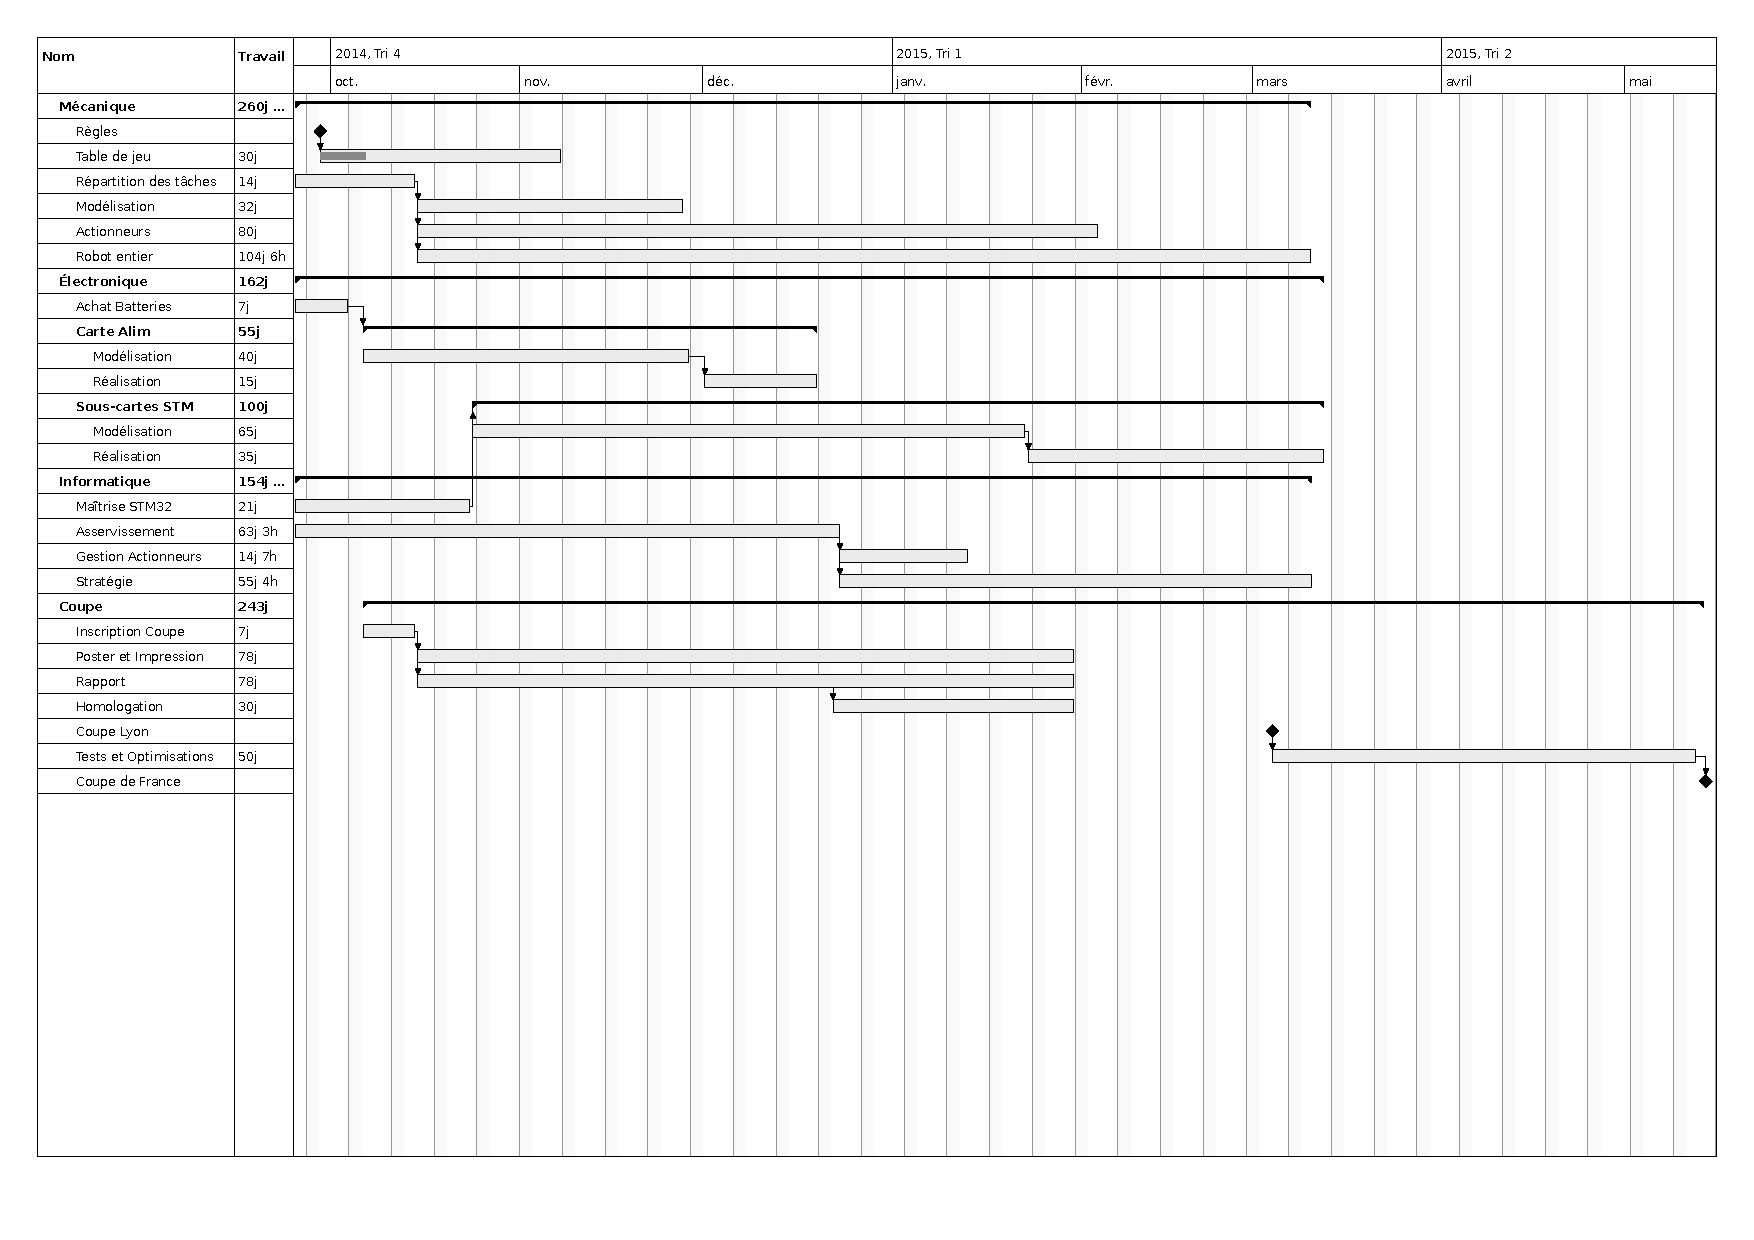
\includegraphics[trim=27px 215px 17px 33px,clip=true , width=\textwidth]{Public/GanttRobo.pdf}
        \caption{Gantt du Club Robotronik} \end{center} \end{figure}

L'échéancier se divise naturellement en trois catégories (en ce qui concerne la partie technique) que sont les composantes du club : mécanique, électronique et informatique.

Les trois parties ne sont bien entendu pas indépendantes, mais nous pouvons débuter chacune séparément, afin de préparer certains aspects de l'informatique qui ne dépend pas des robots -- mais qui doivent être refait avec les changements techniques décidés -- ou les cartes de protection des batteries côté Électronique.\\

La modélisation de la mécanique pose les bases nécessaires au dimensionnement de l'électronique, mais bien sûr nous serons confrontés à des problèmes de réalisation. C'est pourquoi nous devons avancer au plus vite sur la mécanique pour déterminer les modifications à effectuer sur l'électronique, et pour permettre à l'informatique d'être finalisée, évaluée et calibrée.\\


Le temps que je dois consacrer au club comprend la participation à la fabrication, à laquelle je participe bien sûr, mais aussi la gestion de tous les aspects administratifs du Club.

C'est pourquoi le Club me prend 7 à 8 heures par semaine tout au long de l'année, en comptant 5h30 de présence au club.

De plus, nous aurons à passer plus de temps en fin d'année sur la réalisation des robots, je peux estimer à 10 heures par semaine mon investissement au club.\\

J'estime donc à 270 heures le temps que je destine au Club, sans compter la Coupe qui se déroule sur cinq jours mi-Mai.

\part{Points de suivi et contenus présentables}
Le principal "Milestone" est bien sûr la Coupe de France, mi-Mai. Mais comme je l'ai dit plus haut, nous l'avons avancé à la pré-coupe de Lyon en Mars, qui nous permettra de visualiser les différents problèmes de nos robots avant la Coupe.\\

De plus, plusieurs points clés peuvent être retrouvés tout au long de l'année.

Notamment ce vendredi a été finalisé le char de Phelma pour les Ol'INPiades, pour lequel nous avons fait des yeux lumineux ; Samedi a eu lieu la Fête de la Science, pour laquelle nous avons eu à préparer des animations avec le Nao, une imprimante 3D et un des robots qui ont participé à la Coupe l'an dernier.

Ensuite, nous devons finir la table de jeu début novembre, et les cartes de gestion des nouvelles batteries LiPo devront être "livrables" mi-décembre.\\

Côté administratif, je dois préparer pour le Conseil de l'école, le 27 novembre, la présentation du budget du club. Je dois aussi préparer un dossier technique à l'attention des organisateurs de la Coupe, leur permettant d'analyser au plus tôt les erreurs d'interprétation du règlement.

Ce dossier permettra alors de faire un point sur l'avancement du club.

\newpage
\begin{center}
\pagenumbering{roman}
\addcontentsline{toc}{part}{Annexes}
\setcounter{page}{0}
\vspace*{10cm}
{\huge\bfseries Annexes\\
[0.4cm]}\rule{\linewidth}{0.5mm}
\end{center}

\newpage

\section{Organigramme du Club Robotronik}

\vspace*{3cm}
\begin{center}
\begin{tikzpicture}
\tikzstyle{bureau}=[rectangle, minimum height=1.8em,fill=yellow!30,text=black]
\tikzstyle{respo}=[rectangle, minimum height=1.8em,fill=blue!20,text=black]
    \node[bureau] (Prez) at (0,0) {Félix Piédallu, Président};
    \node[bureau] (Trez) at (-5,-1) {Ojeme Ikhalo, Trésorier};
    \node[bureau] (Secr) at (+5,-1) {Florence André, Secrétaire};
    \node[respo] (Chef) at (+0,-2.3) {Johan Lafon, Chef de Projet};
    \node[respo] (Elec) at (-5,-4) {Robin Moussu, Respo Électronique};
    \node[respo] (Info) at (+0,-5) {Robin Moussu, Respo Informatique};
    \node[respo] (Meca) at (+5,-4) {Florence André, Respo Mécanique};
    
    
\tikzstyle{ens}=[<->,dotted,very thick,>=latex]
\tikzstyle{sup}=[<->,dotted,very thick,>=latex]
    \draw[ens] (Chef) -- (Meca);
    \draw[ens] (Chef) -- (Info);
    \draw[ens] (Chef) -- (Elec);
    
    \draw[sup] (Trez) -- (Prez);
    \draw[sup] (Secr) -- (Prez);
    
    \draw[sup] (Prez) -- (Chef);
    \draw[sup] (Trez) -- (Chef);
    \draw[sup] (Secr) -- (Chef);
\end{tikzpicture}
\end{center}
\vspace*{7cm}
\begin{figure}[h]
    \begin{flushright}
        Le Président, Félix Piédallu, le 9 Octobre 2014,\\
        
\includegraphics[width=100px]{Public/SignaturePresident}
    \end{flushright}
\end{figure}

\section{Liens utiles}
\begin{itemize}
    \item \url{http://robotronik.org} Le site du Club Robotronik.
    \item \url{http://wiki.robotronik.org} Le Wiki, public, mis en place début Septembre.
    \item \url{http://www.planete-sciences.org/robot/index.php?section=pages&pageid=125}\\ Le Règlement de la Coupe de France de Robotique 2015.
\end{itemize}

\end{document}
